\section{Extreme Programming explained}
\Alexander{Extreme Programming vs. eXtreme Programming}
% 2 XP's: 2000 and 200? - differences.
% General introduction to XP2k
Extreme Programming (XP) is a software development methodology created by Kent Beck, and this section is based on his book \textit{Extreme Programming Explained (1999)} \citep{xp:explained}. 
Extreme Programming is supposed to be a lightweight, efficient, and fun approach to developing software.

\noindent The methodology consists of the 12 practices:

\begin{tabularx}{\textwidth}{X X X}
	40-hour Week				 & Coding Standards & Collective Ownership \\
	Continuous Integration	  & Metaphor         	 & On-site Customer     \\
	Pair Programming			& Planning Game		& Refactoring          \\
	Simple Design          		  & Small Releases   	& Testing             
\end{tabularx}

Some of these practices are more engrained than others. 
While some supports each other, others may be unrelated. (i.e. coding standards supports collective ownership, but on-site customer and pair programming are unrelated.) The complete map can be seen here:
\begin{figure}[H]
	\centering
	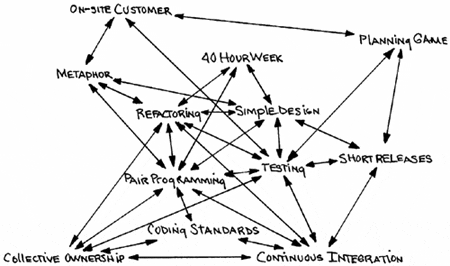
\includegraphics[]{Images/xpPracticeSupport.png}
		\caption{Map, from page 70 in \textit{Extreme Programming Explained (1999)} \citep{xp:explained}, of the practices and how they support each other. }
	\label{fig:practiceSupport}
\end{figure}



\subsection{40-hour Week}
%Why
This practice is created to ensure the developers are well rested and fresh when they come in to work.

%How/What
As the name suggests, the practice encourages developers not to work more than 40 hours per week. 
Although this practice is called 40-hour Week, it should not necessarily be specified to 40 hours per week.
The correct week length will depend on the specific team.

%Coherent
This practice is basis for many of the other practices, as one needs to be well rested to think straight and be creative.
On the other hand, for this practice to work it is required that there are enough tasks to solve.
These tasks are created through the Planning Game practice, hence making it a prerequisite for the 40-hour Week practice to work. 

\subsection{Coding Standards}
%Why
When a project is written by many different developers, it is important that the code are easily understood by other developers.
Otherwise it would waste a lot of time every time a developer has to extend existing code.

%How/What
The practice is all about writing code in a agreed upon format.
This ensure the code are consistent and easy for all developers to understand.

%Coherent
This practice encourages the Collective Ownership, Pair Programming, and Refactoring practice.
%Collective
By making it impossible to distinguish between who wrote what code, it eliminates the tendency to say ``I don't understand this, it is not my code”. Instead the developer instantly understands the purpose, as it is written in a format he understands.\\
%Pair
Pair Programming in and of itself is challenging enough. If you additionally do not understand each others way of coding, it becomes almost impossible. 
A mutual Coding Standard helps by eliminating this problem.\\
%Refactor
It is much faster to refactor a code snippet when you understand its purpose right away.

\subsection{Collective Ownership}
%Why
Extreme Programming strives to be efficient.
Therefore it has adopted a collective approach to ownership, instead of the individual approach.
Where the individual approach enforces stable code, it also leads to slow changes and less code understanding.
In contrast the collective approach enforces rapid changes and high quality, given it is used correctly and does not become ``when everybody is responsible, no one is responsible”.

%How/What
The Collective Ownership works by allowing everybody the rights to change and extend everything.
However, before any changes are released it has to pass 100\% of the automated tests.
If it does not pass, the changes will be discarded, and you try again or let someone else try.

%Coherent
For this to work, it is highly dependent upon the Testing practice, as it is crucial to have very good tests.
Otherwise the changes might break the system and this risk increases every time a change is introduced without being tested.

\subsection{Continuous Integration}
%Why
To avoid wasting time on developing fragmented versions of the same functionality, it is important to integrate at least once a day, often more frequent.

%How/What
When a pair is done with a task, they sit down and integrate it.
They then make sure all unit tests run at 100\%.
If the unit tests does not reach a 100\%, they know it is their task that caused this.
It is therefore up to them to fix it or discard their solution and try again.

%Coherent
It is evident that this practice requires the Testing practice to work.

\subsection{Metaphor}
%Why
The goal of the Metaphor practice is to ensure all developers are on the same page and have the same vision as of what to develop.

%How/What
This is done by creating a metaphor for the system e.g. ``A pacer that plays music in the current tempo”.

%Coherent


\subsection{On-site Customer}
%Why
Huge amounts of time go into analysing the problem domain, without any certainty of it being correct or still applicable throughout the development process.
The On-site Customer practice is implemented to counter this time consuming problem.

%How/What
This is done by making the customer sit in on the actual team.
Here the customer will have to answer questions from the developers and prioritise important features from his point-of-view.

%Coherent


\subsection{Pair Programming}
%Why
Pair Programming is maybe the most controversial practice in Extreme Programming.
When it works it generates high quality code, but when it doesn't it is counterproductive.

%How/What
Pair Programming works with two developers sitting at the same computer.
Here they work together on the same code.
One codes while the other thinks ahead and abstract.


%Coherent
This practice requires a lot of the developers as human beings.
However, when it works it contributes to the Collective Ownership and Simple Design practices as well as general code quality.

\subsection{Planning Game}
%Why
The Planning Game practice is an attempt make the development schedule a collaboration between customer and developer.


%How/What
The Planning Game uses story cards, which are written by the customer.
The story cards describe what the system needs to do and the purpose of the story.
When a story card is written, the developers will estimate its time to implement.
When the stories are estimated, the customer is tasked to decide in which order the stories should be implemented.\\

%Coherent
By planning this way, it enforces the Small Releases practice.

\subsection{Refactoring}
%Why
One of Extreme Programmings core ideals is to \texttt{be brave}.
This means one should not be afraid to refactor working code, if it is to improve the quality of the code.

%How/What
When a developer discovers a method to improve, he does so.
When the refactoring is done, the tests are run and if all pass, the changes are committed to the project.

%Coherent


\Alexander{Spørgsmål til Ivan: Hvilken struktur er bedst, den lange eller den korte?}



\paragraph{Simple Design} is the practice that defines the best design as the easiest that work.
For it to work, it must pass all unit tests and acceptance tests.
Further the best design should be so simple it never has any duplicate code.


\paragraph{Small Releases} are small and frequently versions of the software, which are tested by the customer.
These releases does incrementally complete the system.

\paragraph{Testing} is a mindset, in which, unit tests are developed before the code (Test-First Development).
Testing also refers to how the stories and releases are not complete before they pass their respective tests.


